\documentclass[a4paper, 12pt]{article}

%=========
% PACKAGES
%=========

\usepackage{graphicx}
\usepackage[section]{placeins}
\usepackage{float}
\usepackage{amsmath}
\usepackage{listings}
\usepackage{xcolor}
\usepackage{extarrows}
\usepackage{verbatim}
\usepackage{enumerate}
\usepackage{enumitem}
\usepackage{eurosym}
\usepackage{svg}
\usepackage{varwidth}
\usepackage{moreverb}
\usepackage{relsize}
\usepackage{tabto}
\usepackage[margin=1in]{geometry}
\usepackage[normalem]{ulem}
\usepackage{units}
\usepackage{fancyvrb}
\usepackage{fontspec}
\usepackage{extarrows}
\usepackage{amsfonts}
\usepackage{amssymb}
\usepackage{hyperref}
%\usepackage{unicode-math}


%=====================
% SETTINGS/DEFINITIONS
%=====================

% Don't break words with hyphens. Instead, wrap word to next line.
\tolerance=1
% \emergencystretch=\maxdimen
\hyphenpenalty=10000
\hbadness=10000

\definecolor{codegreen}{rgb}{0,0.6,0}
\definecolor{codegray}{rgb}{0.5,0.5,0.5}
\definecolor{codepurple}{rgb}{0.58,0,0.82}
\definecolor{backcolour}{rgb}{0.95,0.95,0.92}

\def\verbatimtabsize{4}

\lstdefinestyle{mystyle}{
	backgroundcolor=\color{backcolour},
	commentstyle=\color{codegreen},
	keywordstyle=\color{magenta},
	numberstyle=\tiny\color{codegray},
	stringstyle=\color{codepurple},
	basicstyle=\ttfamily\footnotesize,
	breakatwhitespace=false,
	breaklines=true,
	captionpos=b,
	keepspaces=true,
	numbers=left,
	numbersep=5pt,
	showspaces=false,
	showstringspaces=false,
	showtabs=false,
	tabsize=2
}

\lstset{style=mystyle}

\setlength{\parindent}{0pt}
\setlength{\parskip}{0em}
\setlength{\jot}{4mm}

\pagenumbering{gobble}

\hypersetup{
    colorlinks=true,
    linkcolor=blue,
    filecolor=blue,      
    urlcolor=blue,
}

\setmainfont{Minion Pro}

\newcommand{\imagesPath}{.}

\title{
	\textbf{Επεξεργασία Φωνής και Φυσικής Γλώσσας} \\~\\
	2η εργαστηριακή άσκηση \\ 
	Αναγνώριση φωνής με το Kaldi Toolkit
}

\author{
	Ηλίας Κουμουκέλης, el18157 \\
	Νικόλαος Παγώνας, el18175
}

\date{}

\begin{document}

\maketitle
% \textcolor{red}{ και στο βήμα 4 το ερώτημα 1 να γράψω κάτι πράγματα και οι φώτο, στο ερώτημα 3 θέλει πινακάκια }
        
\section*{1 Εισαγωγή}
    Ο κώδικας που έχει γραφτεί έχει δοκιμαστεί με Python \verb|3.7.13|. Προτείνεται τα αρχεία python να εκτελεστούν σε ένα καινούργιο environment με την έκδοση αυτή, για να μην υπάρξουν θέματα με τυχόν πακέτα/βιβλιοθήκες. \\
    
    Ο κώδικας που έχουμε γράψει βρίσκεται στον φάκελο \verb|usc/scripts/| (εκτός από το \verb|main.sh| που βρίσκεται έξω από το \verb|scripts/|, στον \verb|usc/|) και είναι χωρισμένος σε βήματα:
    
    \begin{itemize}
        \item \verb|3.py|
        \item \verb|4.1.py|
        \item \verb|4.2.py|
        \item \verb|4.3.py|
        \item \verb|4.4.py|
    \end{itemize}
    
    Για να εκτελεστεί όλος ο κώδικας μαζί, πρέπει να εκτελεστεί το \verb|main.sh| μέσα από τον φάκελο \verb|usc/| (επομένως η εντολή \verb|pwd| πρέπει να εκτυπώνει \verb|path/to/usc/|, αλλιώς θα υπάρξουν σφάλματα κατά την εκτέλεση). \\
    
    Επιπλέον, η default συμπεριφορά του \verb|main.sh| είναι να ξανακατεβάζει τόσο τα δεδομένα από το Google Drive link, όσο και τα απαραίτητα αρχεία από το \href{https://github.com/slp-ntua/slp-labs/}{slp-ntua/slp-labs}. Προτείνουμε να διατηρήσετε αυτή τη συμπεριφορά. Τα αρχεία κάνουν λίγα δευτερόλεπτα για να κατέβουν, και έτσι εξασφαλίζεται ότι το \verb|main.sh| θα βρει τα αρχεία που χρειάζεται στα σωστά σημεία. \\
    
    Τέλος, έχουμε γράψει κάποια convenience scripts, τα οποία χρησιμοποιούν τα παραπάνω αρχεία-βήματα:
    
    \begin{verbatim}
build-lm-wrapper.sh       # source path.sh before calling build-lm.sh
clean.sh                  # clean everything except main.sh and scripts/
compile-lm-wrapper.sh     # source path.sh before calling compile-lm.sh
download.sh               # download dependencies (Google Drive/GitHub)
helpers.py                # for running bash commands from within python
prepare_lang-wrapper.sh   # source path.sh before calling prepare_lang.sh
timit_format_data.sh      # taken from timit/ recipe
    \end{verbatim}

\section*{2 Θεωρητικό υπόβαθρο}

    \subsection*{Mel-frequency Cepstral Coefficients (MFCCs)}
    
    Στην αναγνώριση φωνής ένας από τους πιο γνωστούς τρόπους για την εξαγωγή χαρακτηριστικών και την αναπαράσταση τους είναι τα MFCCs. Τα Mel Frequency Cepstral Coefficients είναι βασισμένα στο Cepstrum (αντίστροφος μετασχηματισμός Fourier του λογαρίθμου του εκτιμώμενου σήματος). Η διαδικασία εξαγωγής των χαρακτηριστικών είναι η εξής:
    
        \begin{itemize}
            \item \textbf{Pre-Emphasis:} Ο σκοπός σε αυτό το βήμα είναι η ενίσχυση των υψηλών συχνοτήτων, επειδή η ενέργεια στις υψηλές συχνότητες των φωνηέντων είναι αρκετά μικρότερη σε σχέση με τις χαμηλές. Αυτό έχει αποτέλεσμα να εντοπίζονται πιο εύκολα, και έτσι βελτιώνεται η ακρίβεια του μοντέλου.
    
            \item \textbf{Framing and Windowing:} Η ομιλία είναι ένα μη στατικό δείγμα, επομένως αν υπολογίσουμε τον μετασχηματισμό Fourier σε όλο το σήμα δεν μπορούμε να εξάγουμε φασματικά χαρακτηριστικά, αφού χάνεται μεγάλη πληροφορία του φάσματος. Συνεπώς, επιλέγουμε ένα μικρό χρονικό παράθυρο, στη διάρκεια του οποίου εφαρμόζουμε τη συνάρτηση παραθύρου. Συνήθως χρησιμοποιούμε το παράθυρο Hamming, το οποίο -όπως φαίνεται στο παρακάτω σχήμα- έχει μια σταθερή ομαλοποίηση στις άκρες του, και έτσι δεν χάνεται  πληροφορία στην αρχή και στο τέλος του. 
            
            \begin{figure}[H]
                \begin{center}
                    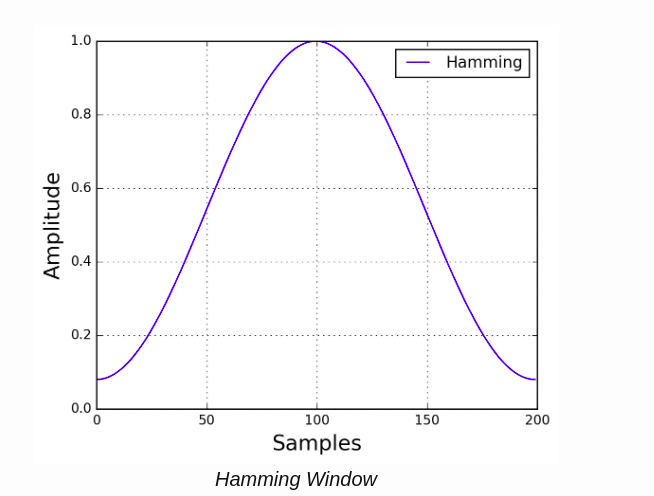
\includegraphics[height=10cm]{hamming.png}
                \end{center}
            \end{figure}

            \item \textbf{Fourier-Transform:} Έπειτα υλοποιούμε τον Διακριτό Μετασχηματισμό Fourier μέσω του FFT-$N$ σημείων (σε όλα τα παράθυρα πλήθους $N$) και παίρνουμε τον Short-Time-Fourier-Τransform ολόκληρου του σήματος. 
    
            \item \textbf{Mel-filter-bank:} Ο τρόπος που τα αυτιά μας αντιλαμβάνονται τον ήχο δεν είναι γραμμικός, οπότε οι αλλαγές στις χαμηλές συχνότητες είναι πιο αισθητές σε σχέση με τις υψηλές. Η κλίμακα Mel μετατρέπει τις συχνότητες λαμβάνοντας υπόψιν αυτή την ιδιαιτερότητα. Έχει παρατηρηθεί ότι η εφαρμογή της στην εξαγωγή χαρακτηριστικών βελτιώνει την αναγνώριση φωνής σε θορυβώδη σήματα.
            
            \item \textbf{DCT:} Ο διακριτός μετασχηματισμός συνημιτόνου εκφράζει μία  πεπερασμένη ακολουθία δεδομένων ως άθροισμα συνημιτόνων διαφορετικών συχνοτήτων. Σε αντίθεση με τον μετασχηματισμό Fourier, δεν έχει φανταστικές συνιστώσες, με αποτέλεσμα να είναι πιο γρήγορος ο υπολογισμός του. Παρά το γεγονός ότι έχει μόνο πραγματικές τιμές, έχει αποδειχθεί ότι δεν χάνει πληροφορία από το σήμα γιατί είναι γραμμικός. Με την εφαρμογή του στον λογάριθμο της κλίμακας Mel παίρνουμε 13 cepstral συντελεστές deltas και deltas-deltas (πρώτη και δεύτερη παράγωγος των MFCCs αντίστοιχα).
            
        \begin{figure}[H]
            \begin{center}
                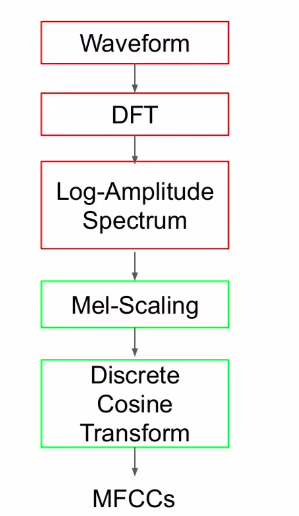
\includegraphics[width=0.5\linewidth]{mfccs.png}
            \end{center}
        \end{figure}
        
        \end{itemize}   

    
    \subsection*{Γλωσσικά Μοντέλα (Language Models)}
    
        Τα γλωσσικά μοντέλα καθορίζουν την πιθανότητα μίας λέξης με χρήση ανάλυσης δεδομένων. Για να γίνει η διάκριση ανάμεσα σε λέξεις και προτάσεις που είναι ομόηχες χρησιμοποιεί διάφορες πιθανοτικές προσεγγίσεις και επιλέγει τον συνδυασμό λέξεων που είναι πιο πιθανός σε μια πρόταση. Μερικές από αυτές τις προσεγγίσεις είναι:
      
        \begin{itemize}
            \item \textbf{Ν-gram}: Δημιουργεί μία πιθανοτική κατανομή για μια ακολουθία από $N$ στοιχεία. 
        
        \begin{align*}
            P(w_{1:n}) &= P(w_1)P(w_2|w_1)P(w_3|w_{1:2})...P(w_n|w_{1:n-1}) \\
                      &= \prod_{k=1}^{n} P(w_k|w_{1:k-1})
        \end{align*}
            
            \item \textbf{Unigram και Bigram}: Αποτελούν ειδικές περιπτώσεις του $n$-gram με $n = 1$ και $n = 2$ και είναι και αυτά που χρησιμοποιήσαμε στην εργασία. Στο bigram η κάθε λέξη εξαρτάται από μία προηγούμενη κατάσταση ενώ στο unigram από την a-priori πιθανότητα εμφάνισης της λέξης. \\
            
            \textbf{Unigram:}
            
            \[
                P ( w_n | w_1,w_2,..,w_n ) = P(w_n)
            \] 
            
            
            \textbf{Bigram:} 
            
            \[
                P(w_n|w_1,w_2,...,w_n) = P(w_n|w_{n-1})
            \]
        \end{itemize}
    
    \subsection*{Φωνητικά Μοντέλα (Acoustic Models)}
        Τα φωνητικά μοντέλα αποτελούν αναπαραστάσεις του σήματος σε φωνήματα. Με βάση τις Γκαουσιανές μίξεις, παράγονται ορισμένα γνωρίσματα τα οποία αποτελούν τα χαρακτηριστικά του φωνητικού μοντέλου. Στην εκπαίδευση, κάθε πρόταση διασπάται σε επιμέρους λέξεις και κάθε λέξη στα αντίστοιχα φωνήματα, και έτσι δημιουργούνται οι αναπαραστάσεις. Επομένως γίνεται η εκτίμηση των παραμέτρων μεταξύ των καταστάσεων του μοντέλου και δημιουργείται ένας πίνακας μεταβάσεων κάθε φωνήματος και οι πιθανότητες των παρατηρήσεων που αποτελούν τα Hidden Markov Models (HMMs). Τέλος, με την υλοποίηση του αλγορίθμου forward-backward γίνεται η εκτίμηση για το ποια είναι η πιθανή ακολουθία φωνημάτων, ώστε να γίνει η αναγνώριση. 
        
        \begin{figure}[H]
            \begin{center}
                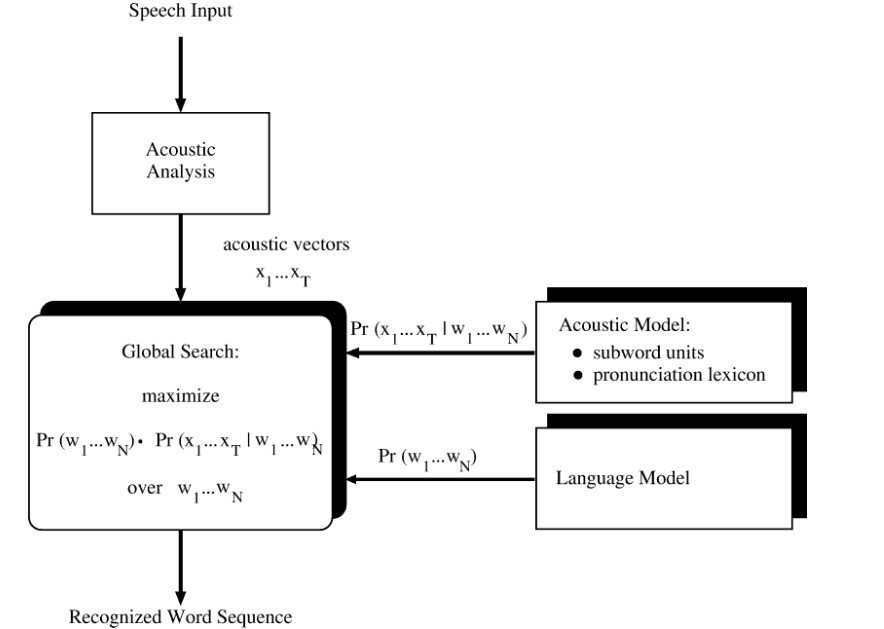
\includegraphics[width=\linewidth]{hmm.png}
            \end{center}
        \end{figure}

\section*{3 Βήματα προπαρασκευής}
    
    \subsection*{1.}
        Εγκαθιστούμε το Kaldi σύμφωνα με τις οδηγίες που μας δίνονται.
        
    \subsection*{2.}
        Εξοικειωνόμαστε με το Kaldi, με βάση τα tutorials που δίνονται.
    
    \subsection*{3.}
        Με χρήση του \verb|download.sh|, κατεβάζουμε τα δεδομένα από το Google Drive link που μας δίνεται.
    
    \subsection*{4.}
        Με χρήση του \verb|3.py| κατασκευάζουμε τον αρχικό σκελετό ως εξής:
        
        \begin{itemize}
            \item Μέσα στον φάκελο \verb|egs/| δημιουργούμε έναν φάκελο \verb|usc/|.
            
            \item Δημιουργούμε τον φάκελο \verb|data| και τους υποφακέλους \verb|data/train, data/dev, data/test|.
            
            \item Μέσα σε καθέναν από αυτούς τους 3 φακέλους δημιουργούμε τα αρχεία:
                \begin{itemize}
                    \item \verb|uttids|
                    \item \verb|utt2spk|
                    \item \verb|wav.scp|
                    \item \verb|text|
                \end{itemize}
                
                Η μορφή και η χρήση τους περιγράφεται αναλυτικά στην εκφώνηση της άσκησης.
            
            \item Με χρήση του \verb|lexicon.txt| αντικαθιστούμε τις λέξεις των προτάσεων με τις αντίστοιχες ακολουθίες φωνημάτων. Για τον σκοπό αυτό μετατρέπουμε όλους τους χαρακτήρες σε lower case και αφαιρούμε τους ειδικούς χαρακτήρες, εκτός από τα single quotes. Επίσης προσθέτουμε το φώνημα \verb|sil| (σιωπή) στην αρχή και στο τέλος της κάθε πρότασης.
        \end{itemize}

\section*{4 Βήματα κυρίως μέρους} 
    
    \subsection*{4.1 Προετοιμασία διαδικασίας αναγνώρισης φωνής για τη USC-TIMIT}
    
        Με χρήση του \verb|4.1.py| εκτελούμε τα βήματα που ακολουθούν:
        
        \subsubsection*{1.}
            Από τη διαδικασία \verb|wsj/| παίρνουμε τα αρχεία \verb|path.sh| και \verb|cmd.sh|. Στο \verb|path.sh|, θέτουμε κατάλληλα τη μεταβλητή \verb|KALDI_ROOT| και στο \verb|cmd.sh|  θέτουμε τις μεταβλητές \verb|train_cmd, decode_cmd| και \verb|cuda_cmd| ίσες με \verb|run.pl|.
        
        \subsubsection*{2.}
            Δημιουργούμε soft links με ονόματα \verb|steps| και \verb|utils| μέσα στο φάκελο \verb|usc/|, που δείχνουν στους αντίστοιχους φακέλους της \verb|wsj|.
        
        \subsubsection*{3.} 
            Δημιουργούμε τον φάκελο \verb|local|, και μέσα σ'αυτόν ένα soft link με όνομα \verb|score.sh| που δείχνει στο \verb|steps/score_kaldi.sh|. 
        
        \subsubsection*{4.} 
            Δημιουργούμε τον φάκελο \verb|conf/| και μέσα σε αυτόν αντιγράφουμε το αρχείο \verb|mfcc.conf| που βρίσκεται στο \href{https://github.com/slp-ntua/slp-labs/blob/master/lab2/mfcc.conf}{slp-ntua/slp-labs}.
        
        \subsubsection*{5.}
            Τέλος, δημιουργούμε τους φακέλους:
            
            \begin{verbatim}
data/lang, data/local/dict, data/local/lm_tmp, data/local/nist_lm
            \end{verbatim}
        
    \subsection*{4.2 Προετοιμασία γλωσσικού μοντέλου}
    
        Με χρήση του \verb|4.2.py| εκτελούμε τα βήματα που ακολουθούν:
    
        \subsubsection*{1.}
            Αρχικά στον φάκελο \verb|data/local/dict| αποθηκεύουμε τα βασικά αρχεία που χρησιμεύουν για τη δημιουργία του γλωσσικού μοντέλου.
            
            \begin{itemize}
                \item \verb|silence_phones.txt| και \verb|optional_silence.txt|, που περιέχουν μόνο το φώνημα της σιωπής \verb|(sil)|.
                
                \item Το \verb|nonsilence_phones.txt| το οποίο περιέχει όλα τα υπόλοιπα φωνήματα ταξινομημένα, και ένα σε κάθε γραμμή.
                
                \item Το \verb|lexicon.txt|, το οποίο στην δική μας περίπτωση είναι απλά μία 1-1 αντιστοιχία κάθε φωνήματος με τον εαυτό του.
                
                \item Τα \verb|lm_{train,dev,test}.text|, που προκύπτουν από τα αντίστοιχα αρχεία \verb|text| (βλ. προπαρασκευή), αν προσθέσουμε σε κάθε πρόταση τα \verb|<s>| και \verb|</s>| στην αρχή και στο τέλος αντίστοιχα.
                
                \item Τέλος, δημιουργούμε το (κενό) αρχείο \verb|extra_questions|.
            \end{itemize}
        
        \subsubsection*{2.}
            Μέσα στον φάκελο \verb|data/local/lm_tmp| δημιουργούμε την ενδιάμεση μορφή του γλωσσικού μοντέλου. Συγκεκριμένα, θα χρησιμοποιήσουμε την εντολή \verb|build-lm.sh| του πακέτου \verb|IRSTLM|. Για τον σκοπό αυτό δημιουργούμε το αρχείο \verb|build-lm-wrapper.sh|, το οποίο κάνει source το \verb|path.sh| ώστε να γίνει διαθέσιμη η εντολή \verb|build-lm.sh|, και ύστερα την καλεί. Δημιουργούμε τόσο unigram όσο και bigram μοντέλα βάζοντας την παράμετρο \verb|-n| ίση με $1$ και $2$ αντίστοιχα.
        
        \subsubsection*{3.}
            Μέσα στον φάκελο \verb|data/local/nist_lm| αποθηκεύουμε το compiled γλωσσικό μοντέλο σε μορφή ARPA. Για τον σκοπό αυτό δημιουργούμε το αρχείο \verb|compile-lm-wrapper.sh|, το οποίο κάνει source το \verb|path.sh| ώστε να γίνει διαθέσιμη η εντολή \verb|compile-lm.sh|, και ύστερα την καλεί. Προκύπτουν τα αρχεία \verb|lm_phone_ug.arpa.gz| (unigram μοντέλο) και \verb|lm_phone_bg.arpa.gz| (bigram μοντέλο).
        
        \subsubsection*{4.}
            Μέσα στον φάκελο \verb|data/lang| δημιουργούμε το \verb|L.fst| (FST του λεξικού της γλώσσας). Για τον σκοπό αυτό δημιουργούμε το αρχείο \verb|prepare_lang-wrapper.sh|, το οποίο κάνει source το \verb|path.sh| ώστε να γίνει διαθέσιμη η εντολή \verb|prepare_lang.sh|, και ύστερα την καλεί.
        
        \subsubsection*{5.}
            Χρησιμοποιούμε την εντολή \verb|sort| για να ταξινομήσουμε τα αρχεία \verb|wav.scp, text, utt2spk| στους φακέλους \verb|data/{train,dev,test}|.
            
        \subsubsection*{6.}
            Εκτελούμε το \verb|utils/utt2spk_to_spk2utt.pl| και έτσι δημιουργούμε το αρχείο \verb|spk2utt|.
            
        \subsubsection*{7.}
            Τέλος, δημιουργούμε το \verb|G.fst| (FST της γραμματικής), με βάση τη διαδικασία \verb|timit| (αρχείο \verb|local/timit_format_data.sh|).

        \subsubsection*{Ερώτημα 1: Για τα γλωσσικά μοντέλα που δημιουργήσατε υπολογίστε το perplexity στο validation και στο test set. Τι δείχνουν αυτές οι τιμές;} 
        
        Το Perplexity είναι η μέτρηση για το πόσο καλά μια πιθανοτική κατανομή μπορεί να προβλέψει ένα δείγμα και δείχνει το πόσο περιπλέκεται το μοντέλο μας (όσο μικρότερο τόσο το καλύτερο). Έχουμε: \\
        
        \begin{center}
            \begin{tabular}{|c|c|c|}
                \hline
                              & \textbf{Unigram} & \textbf{Bigram} \\ \hline
                \textbf{Dev}  & 56.23            & 27.02  \\ \hline
                \textbf{Test} & 55.15            & 26.39  \\ \hline
            \end{tabular}    
        \end{center}
        
        
        Παρατηρούμε ότι το bigram αποδίδει πολύ καλύτερα από το unigram (το perplexity πέφτει σχεδόν στο μισό). Αυτό είναι λογικό, γιατί το unigram δεν χρησιμοποιεί την προηγούμενη κατάσταση για να υπολογίσει την πιθανότητα του κάθε φωνηέντου αλλά μόνο την a-priori πιθανότητα εμφάνισης του.
        
    \subsection*{4.3 Εξαγωγή ακουστικών χαρακτηριστικών}
        Με χρήση του \verb|4.3.py| - το οποίο καλεί τις εντολές \verb|make_fcc.sh| και \verb|compute_cmvn_stats.sh| - εξάγουμε τα MFCCs και για τα 3 σετ. 
        
        \subsubsection*{Ερώτημα 2: Με τη δεύτερη εντολή πραγματοποιείται το λεγόμενο Cepstral Mean and Variance Normalization. Τι σκοπό εξυπηρετεί;}
            To CMVN είναι μία υπολογιστικά αποδοτική τεχνική κανονικοποίησης του σήματος που χρησιμοποιείται στην αναγνώριση φωνής. Ο στόχος της εύρωστης εξαγωγής στοιχείων είναι η ελαχιστοποίηση της παραμόρφωσης που δημιουργείται στα σήματα φωνής λόγω του θορύβου, ώστε να γίνεται η βέλτιστη εξαγωγή χαρακτηριστικών. Αυτό επιτυγχάνεται με την κανονικοποίηση της μέσης τιμής και της διασποράς στις τιμές $0$ και $1$ αντίστοιχα. Η κανονικοποίηση αυτή επιτυγχάνει την ομαλοποίηση της διασποράς, επειδή καθώς σχηματίζονται οι συντελεστές, οι μικρές αλλαγές και ο θόρυβος μπορεί να προκαλέσουν μεγάλο variance με αποτέλεσμα λανθασμένη αναγνώριση του φωνήματος. 
            % Έστω $x[n]$ το αρχικό σήμα φωνής δηλαδή η είσοδος τους συστήματος, h[n] η κρουστική απόκριση, και $y[n]$ η σινέλιξη των παραπάνω:
            
            % \[
            %     y[n] = x[n] \ \ast \ h[n]
            % \] 
            
            % Εφαρμόζοντας DFT παίρνουμε το:
            
            % \[
            %     Y[k] = X[k] \cdot H[k]
            % \]
            
            % Στη συνέχεια λογαριθμίζουμε το $Y[k]$:\\
            
            % \textcolor{red}{Θέλει τα μαθηματικά εδώ που με μπέρδεψε, λογικά είναι η αφαίρεση από τις συνιστώσες την μέση τιμή διά την διασπορά}
        
        \subsubsection*{Ερώτημα 3: Πόσα ακουστικά frames εξήχθησαν για κάθε μία από τις 5 πρώτες προτάσεις του training set; Τι διάσταση έχουν τα χαρακτηριστικά;}
        
        
        Με βάση το αρχείο \verb|data/train/utt2num_frames| έχουμε:
        
        \begin{verbatim}
f1_003: 317 frames
f1_004: 371 frames
f1_005: 399 frames
f1_007: 328 frames
f1_008: 464 frames
        \end{verbatim}
        
        Η διάσταση των χαρακτηριστικών προκύπτει από τη σχέση:
        
        \[
            \text{Διάσταση} = 13 \times \left( \frac{\text{Διάρκεια}}{\text{Frame shift}} \right)
        \]
        
        Η διάρκεια βρίσκεται στο αρχείο \verb|data/train/utt2dur|, το frame shift στο \verb|data/train/frame_shift|, ενώ 13 είναι το πλήθος των συντελεστών του Mel-Frequency Cepstrum που κρατάμε κάθε φορά.
        
    \subsection*{4.4 Εκπαίδευση ακουστικών μοντέλων και αποκωδικοποίηση προτάσεων}
        
        Με χρήση του \verb|4.4.py| εκτελούμε τα βήματα που ακολουθούν:
    
        \subsubsection*{1.}
            Με την εντολή \verb|steps/train_mono.sh| εκπαιδεύουμε ένα monophone GMM-HMM ακουστικό μοντέλο πάνω στα \verb|train| δεδομένα.
        
        \subsubsection*{2.}
            Δημιουργούμε το γράφο HCLG σύμφωνα με την γραμματική G του προηγούμενου βήματος. Χρησιμοποιούμε το \verb|utils/mkgraph.sh| (τόσο για unigrams όσο και για bigrams).
            
        \subsubsection*{3.}
            Χρησιμοποιούμε τον αλγόριθμο Viterbi για να αποκωδικοποιήσουμε τις προτάσεις τόσο των validation όσο και των test δεδομένων. Χρησιμοποιούμε το \verb|steps/decode.sh|.
        
        \subsubsection*{4.}
            Χρησιμοποιούμε το \verb|local/score.sh| και τα αποτελέσματα που βρίσκονται στα αρχεία:
            
            \begin{verbatim}
exp/mono/decode_dev_ug/scoring_kaldi/best_wer
exp/mono/decode_dev_bg/scoring_kaldi/best_wer
exp/mono/decode_test_ug/scoring_kaldi/best_wer
exp/mono/decode_test_bg/scoring_kaldi/best_wer
            \end{verbatim}
            
            Η μετρική PER (Phone Error Rate) είναι:
            
            \begin{align*}
                \text{PER} &= 100 \cdot \dfrac{\#\text{insertions} + \#\text{substitutions} + \#\text{deletions}}{\# \text{phonemes}} \\
            \end{align*}
            
            Με βάση τα αποτελέσματα στα παραπάνω αρχεία έχουμε:
            
            \begin{center}
                \textbf{PER for monophone model} \\~\\
                
                \begin{tabular}{|c|c|c|}
                    \hline
                                  & \textbf{Unigram}   & \textbf{Bigram} \\ \hline
                    \textbf{Dev}  & 52.66\%            & 45.98\%         \\ \hline
                    \textbf{Test} & 51.59\%            & 45.01\%         \\ \hline
                \end{tabular}    
            \end{center}
            
            
        
        \subsubsection*{5.}
            Κάνουμε alignment των φωνημάτων χρησιμοποιώντας το monophone μοντέλο (\verb|steps/align_si.sh|), και με βάση αυτά τα alignments εκπαιδεύουμε ένα triphone μοντέλο (\verb|steps/train_deltas.sh|). Δημιουργούμε τον γράφο HCLG και πραγματοποιούμε αποκωδικοποίηση ξανά. Αυτή τη φορά τα αποτελέσματα βρίσκονται στα αρχεία:
            
            \begin{verbatim}
exp/tri1/decode_dev_ug/scoring_kaldi/best_wer
exp/tri1/decode_dev_bg/scoring_kaldi/best_wer
exp/tri1/decode_test_ug/scoring_kaldi/best_wer
exp/tri1/decode_test_bg/scoring_kaldi/best_wer
            \end{verbatim}
            
            Έχουμε:
            
            \begin{center}
                \textbf{PER for triphone model} \\~\\
            
                \begin{tabular}{|c|c|c|}
                    \hline
                                  & \textbf{Unigram}   & \textbf{Bigram} \\ \hline
                    \textbf{Dev}  & 40.00\%            & 36.66\%         \\ \hline
                    \textbf{Test} & 39.07\%            & 35.03\%         \\ \hline
                \end{tabular}    
            \end{center}            
    
            Υπάρχει αρκετά σημαντική βελτίωση σε σχέση με το monophone μοντέλο. Επίσης εδώ υπάρχει μικρότερη διαφορά μεταξύ unigram και bigram μοντέλου.
    
        \subsubsection*{Ερώτημα 4: Εξηγήστε τη δομή ενός ακουστικού μοντέλου GMM-HMM. Τι σκοπό εξυπηρετούν τα μαρκοβιανά μοντέλα στη συγκεκριμένη περίπτωση και τι τα μίγματα γκαουσιανών; Με ποιο τρόπο γίνεται η εκπαίδευση ενός τέτοιου μοντέλου; Περιγράψτε τη διαδικασία εκπαίδευσης ενός μονοφωνικού μοντέλου.}
        
        Τα GMMs είναι ένας τρόπος να προσδιοριστούν και να ομαδοποιηθούν οι καταστάσεις του αυτόματου σε κατηγορίες με βάση την πιθανότητα ενός φωνήματος να βρίσκεται σε μία λέξη. Αν το μοντέλο μας χρησιμοποιούσε μόνο Gaussian-Mixture-Model, αυτό θα σήμαινε ότι θα κατηγοριοποιούσε κάθε φώνημα χωρίς να λαμβάνει υπόψιν προηγούμενες καταστάσεις, οπότε δεν θα μπορούσε να δει αν ταιριάζει κάποια πρόβλεψη στην εκάστοτε λέξη η πρόταση, προκειμένου να ελαχιστοποιήσει την πιθανότητα λάθους. Γι' αυτό χρησιμοποιεί και τα HMMs, στατιστικά μοντέλα τα οποία υποθέτουν κρυφές καταστάσεις (τοποθέτηση γλώσσας, ποια συντακτική θέση έχει η λέξη στην οποία βρίσκεται το φώνημα, πιθανότητες μετάβασης από μία ακολουθία $N$ φωνημάτων σε ένα άλλο). Ο τρόπος που γίνεται η εκπαίδευση είναι με μια ειδική κατηγορία του Expectation-Maximization, τον forward-backward, ο οποίος μας επιτρέπει να υπολογίσουμε την πλήρη υπό συνθήκη πιθανοφάνεια μιας σειράς καταστάσεων, δεδομένης μιας ακουλουθίας παρατηρήσεων. Αρχικά κάνει μια εκτίμηση για την μέση τιμή και διασπορά  των δεδομένων και έπειτα τις ξανά υπολογίζει επαναληπτικά με βάση τις προηγούμενες τιμές και τις καταστάσεις μετάβασης, οπότε μεγαλώνει η πιθανοφάνεια και συγκλίνει σε μία τιμή. Έτσι, εκπαιδεύουμε ταυτόχρονα τόσο τα transition, όσο και τα emission probabilities του ΗΜΜ.
        
        \subsubsection*{Ερώτημα 5: Γράψτε πώς υπολογίζεται η a posteriori πιθανότητα σύμφωνα με τον τύπο του Bayes για το πρόβλημα της αναγνώρισης φωνής. Συγκεκριμένα, πώς βρίσκεται η πιο πιθανή λέξη (ή φώνημα στην περίπτωσή μας) δεδομένης μίας ακολουθίας ακουστικών χαρακτηριστικών;}
        
        Το Μπεϋζιανό μοντέλο για την εύρεση πιθανότητας ενός φωνήματος είναι με βάση την a posteriori για κάθε πιθανό φώνημα δεδομένης μια ακουλουθίας λέξεων και φωνημάτων (χαρακτηριστικών).
        
        \[
            P(W|X) = \frac{P(X|W)\cdot P(W)}{P(X)}
        \]
       
        όπου:
        \begin{itemize}
            \item $P(W|X)$ η a-posteriori πιθανότητα,
            \item $P(X|W)$ η πιθανότητα ανίχνευσης χαρακτηριστικών $Ο$ δεδομένου του φωνήματος $W_i$ επομένως το φωνητικό μοντέλο(acoustic model)
            \item $P(W)$ η a-priori που είναι η πιθανότητα εμφάνισης των χαρακτηριστικών(language model) 
        \end{itemize}
        Έπειτα από τα $i$ πιθανά φωνήματα που έχουν προκύψει, βρίσκουμε την μέγιστη πιθανοφάνεια και προκύπτει το εκτιμώμενο φώνημα. \\
        
        \[
            W = \text{argmax}_{0 \leq i \leq n}\left\{{P(W_i|X)}\right\} = \text{argmax}_{0 \leq i \leq n}\left\{\frac{P(X|W_i)\cdot P(W_i)}{P(X)} \right\}
        \]
    
        Αφού θέλουμε να δούμε για ποιο $W_i$ μεγιστοποιείται η παραπάνω συνάρτηση, μπορούμε να απαλείψουμε τον όρο $P(X)$, γιατί παραμένει ίδιος για όλα τα $i$. Επομένως, έχουμε το εξής:
        
        \[
            W = \text{argmax}_{0 \leq i \leq n} \{P(X|W_i)\cdot P(W_i)\}
        \]
    
        \subsubsection*{Ερώτημα 6: Εξηγήστε τη δομή του γράφου HCLG του Kaldi περιγραφικά.}
    
        O γράφος HCLG είναι αναπτυγμένο γράφημα αποκωδικοποίησης που αναπαριστά τον αποδοχέα γραμματικής, το λεξικό φωνημάτων, τα ΗΜΜs και τα context-dependency. To output είναι ένα fst με word-ids και ως input δέχεται word-ids.
    
        \begin{itemize} 
            \item \verb|Η.fst| είναι το FST που περιέχει πληροφορίες για τα HMMs.
            \item \verb|C.fst| είναι το FST που κάνει τα φωνήματα σε contex-dependency. 
            \item \verb|L.fst| είναι λεξικό που παίρνει ως είσοδο μία λέξη και μας δίνει σαν έξοδο τα επιμέρους φωνήματα. 
            \item \verb|G.fst| είναι ο αποδοχέας της γραμματικής.          
        \end{itemize}
\end{document}